%%%%%%%%%%%%%%%%%%%%%%%%%%%%%%%%%%%%%%%%%%%%%%%%%%%%%%%%%%%%%%%%%%%%%%%%%%%%%%%
\section[Section]{Classical cryptography}
\part{Classical cryptography}

%%%%%%%%%%%%%%%%%%%%%%%%%%%%%%%%%%%%%%%%%%%%%%%%%%%%%%%%%%%%%%%%%%%%%%%%%%%%%%%
\begin{frame}{Caesar cipher}

\centering

\smallskip

Encrypt: right shift each letter of 3 positions

\smallskip

Decrypt: left shift each letter of 3 positions

\medskip

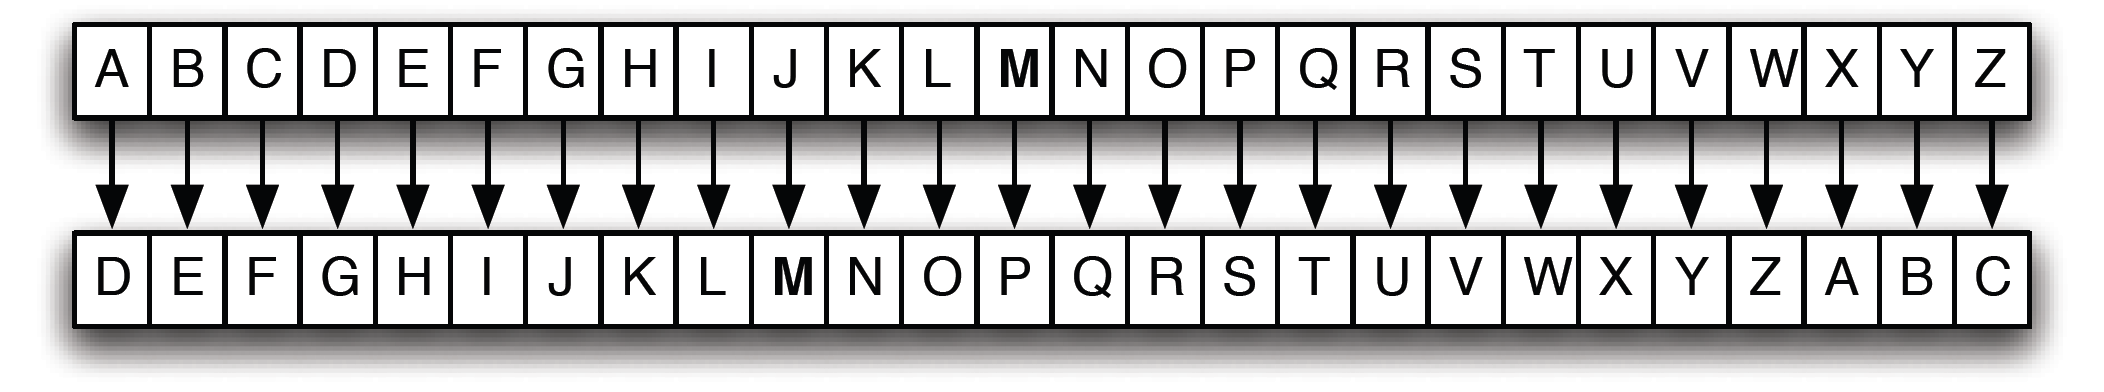
\includegraphics[width=10cm]{img/caesar-shift.png}

\medskip

General cipher: shift letter of $K$ positions

\smallskip

Attack: bruteforce all the possible $K$ (only $26$...)

\end{frame}

%%%%%%%%%%%%%%%%%%%%%%%%%%%%%%%%%%%%%%%%%%%%%%%%%%%%%%%%%%%%%%%%%%%%%%%%%%%%%%%
\begin{frame}{ROT\{13, 47\}}

\centering

\medskip

ROT13: Caesar cipher with $K = 13$ on alphabetic dictionary

ROT47: Caesar cipher with $K = 47$ on printable ASCII chars (33 - 126).

\medskip

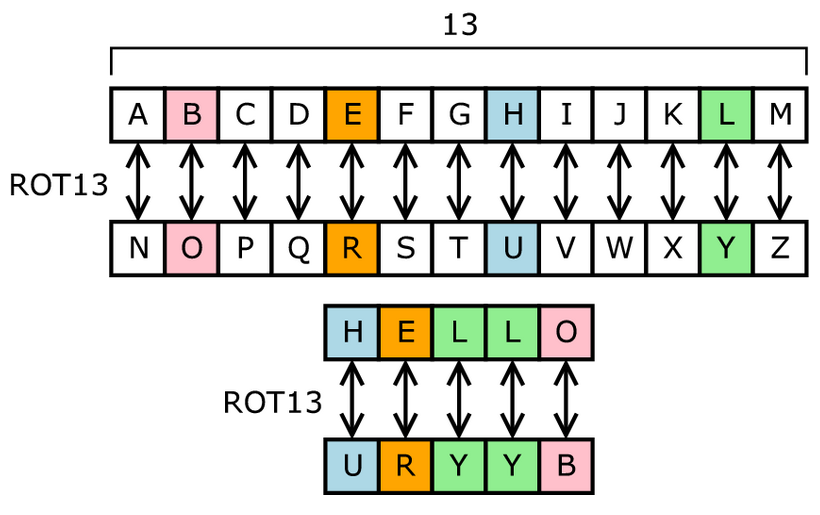
\includegraphics[width=8cm]{img/ROT13.png}

\medskip

Why $K = 13$ (or $K = 47$)? Because Encrypt = Decrypt

\end{frame}

%%%%%%%%%%%%%%%%%%%%%%%%%%%%%%%%%%%%%%%%%%%%%%%%%%%%%%%%%%%%%%%%%%%%%%%%%%%%%%%
\begin{frame}{Classical ciphers}

\textbf{Substitution ciphers}

\textcolor{red}{Monoalphabetic} ciphers: $C_{new} = P[C_{old}]$ (Where $P$ is a dictionary permutation)

\smallskip

(ROT-K is a monoalphabetic cipher where $P$ is a cyclic rotation of the alphabet)

\smallskip

\textcolor{red}{Polialphabetic} ciphers: multiple substitution alphabets (more than one dictionary permutation)

\smallskip

\textbf{Transposition ciphers}

Encryption systems where the positions held by units of plaintext (characters or groups of characters) are shifted according to a regular system.

\smallskip

E.g. We want to encrypt the message \textit{WE ARE DISCOVERED. FLEE AT ONCE} using the \textbf{route cipher}:

Grid: 

\centerline{\texttt{W R I O R F E O E}}
\centerline{\texttt{E E S V E L A N J}}
\centerline{\texttt{A D C E D E T C X}}

Cipher text: \textit{EJXCTEDECDAEWRIORFEONALEVSE}

\end{frame}
%%%%%%%%%%%%%%%%%%%%%%%%%%%%%%%%%%%%%%%%%%%%%%%%%%%%%%%%%%%%%%%%%%%%%%%%%%%%%%%
\begin{frame}{Substituion cipher: XXX}
  
\end{frame}
%%%%%%%%%%%%%%%%%%%%%%%%%%%%%%%%%%%%%%%%%%%%%%%%%%%%%%%%%%%%%%%%%%%%%%%%%%%%%%%
\begin{frame}{Transposition cipher: XXX}

\end{frame}
%%%%%%%%%%%%%%%%%%%%%%%%%%%%%%%%%%%%%%%%%%%%%%%%%%%%%%%%%%%%%%%%%%%%%%%%%%%%%%%
\begin{frame}{dcode.fr}

\centering

\href{https://www.dcode.fr/tools-list}{https://www.dcode.fr/tools-list}

\medskip

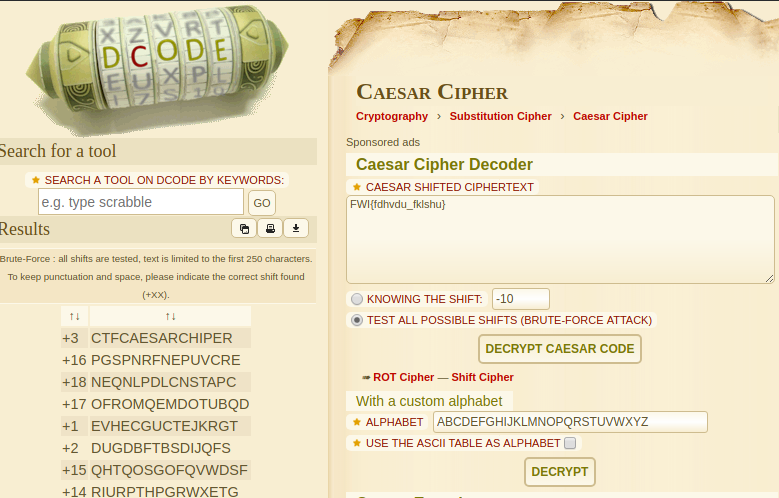
\includegraphics[width=8cm]{img/dcode.png}

\medskip

Almost all possible classic ciphers (old and new), encoder/decoder, ...

\end{frame}
%%%%%%%%%%%%%%%%%%%%%%%%%%%%%%%%%%%%%%%%%%%%%%%%%%%%%%%%%%%%%%%%%%%%%%%%%%%%%%%
\begin{frame}{Cryptanalysis}

Often the vulnerability is not in the algorithm but in its application...

\begin{itemize}
  \item Bad use of the key (too short, reused, bad generated, ...)
  \item Messages use a poorly distributed dictionary
  \item We know the message format (e.g.: \textsc{flag\{\ldots\}})
\end{itemize}

\medskip

In particular we talk about statistical cryptanalysis when we force the cipher not from algorithmic point of view but from statistical one

\medskip

For example in english the character E has a frequency of 12.02\% while Z only 0.07\%

\medskip

Useful tool (for substitution ciphers): \href{https://quipqiup.com}{https://quipqiup.com}

\medskip

\centering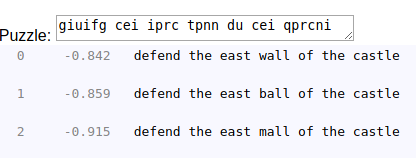
\includegraphics[width=5cm]{img/quipqiup.png}
  
\end{frame}
%%%%%%%%%%%%%%%%%%%%%%%%%%%%%%%%%%%%%%%%%%%%%%%%%%%%%%%%%%%%%%%%%%%%%%%%%%%%%%%

\begin{frame}{Attack models}

Classification of cryptographic attacks:

\medskip

\begin{itemize}
  \item \textcolor{red}{Ciphertext-only} attack: access only to the ciphertext, and has no access to the plaintext
  \medskip
  \item \textcolor{red}{Known-plaintext} attack: access to at least a limited number of pairs of plaintext and the corresponding enciphered text
  \medskip
  \item \textcolor{red}{Chosen plaintext} attack: able to choose a number of plaintexts to be enciphered and have access to the resulting ciphertext (encrypt oracle)
  \medskip
  \item \textcolor{red}{Chosen ciphertext} attack: able to choose arbitrary ciphertext and have access to plaintext decrypted from it (decrypt oracle) 
  \medskip
  \item \textcolor{red}{Side-channel} attack: use of other informations to break the cipher (time, sound, power, error, ...).
\end{itemize}
  
\end{frame}
%%%%%%%%%%%%%%%%%%%%%%%%%%%%%%%%%%%%%%%%%%%%%%%%%%%%%%%%%%%%%%%%%%%%%%%%%%%%%%%
